\documentclass[12pt]{article}
\usepackage[spanish]{babel}

\usepackage{enumerate}
\usepackage{geometry}
\usepackage{graphicx}
	\graphicspath{ {assets/} }
\usepackage{hyperref}
	\hypersetup{ colorlinks=true,
				linkcolor=red,
				urlcolor=cyan,
				filecolor=yellow}
\usepackage{multicol}
\usepackage{amssymb}

%%%%%%%%%%%%%%%%%%%%%%%%%%%%%%%%%%
%%%%%%%%%%%%%%%%%%%%%%%%%%%%%   %%
%%        Datos Trabajo     %%  %%
%%%%%%%%%%%%%%%%%%%%%%%%%%%%%%%%%%
\newcommand{\titulo}[0]{
Actividad 3. Relación entre las dimensiones del desarrollo sustentable}
\newcommand{\materia}[0]{Desarrollo Sustentable}
\newcommand{\grupo}[0]{BI-BDSU-2002-B1-012}
\newcommand{\unidad}[0]{Unidad 2}
%%%%%%%%%%%%%%%%%%%%%%%%%%%%%%%%%%
%%%%%%%%%%%%%%%%%%%%%%%%%%%%%%%%%%

\title{
	
\includegraphics{../../../assets/logo-unadm.png} \\
	\ \\ Benjam\'in Rivera \\
	\bf{\titulo}\\\ \\}

\author{
	Universidad Abierta y a Distancia de México \\
	TSU en Biotecnolog\'ia \\
	\textit{Materia:} \materia \\
	\textit{Grupo:} \grupo \\
	\textit{Unidad:} \unidad \\
	\\
	\textit{Matricula:} ES202105994 }

\date{\textit{Fecha de entrega:} \today}


%%%%%%%%%%%%%%%%%%%%%%%%%%%%%
%%        Documento         %%
%%%%%%%%%%%%%%%%%%%%%%%%%%%%%%%
\begin{document}
\maketitle\newpage

\section*{Proyecto}

	\par El proyecto que yo escogí en la sección anterior se llama Todo ha cambiado para siempre, Este proyecto trata de impulsar distintos metodos de comunicación entre los profesores y sus alumnos, como por ejempli la música y la danza, se guia por la idea de que no todas las cosas pueden comunicarse con palabras.

	\par Este programa es desarrollado en la escuela primaria Al Ribat en Trípoli, que es la capital de Libia, la cual fue fundada en 1969. Este centro educativo cuenta con profesores que realmente estan compormetidos con su labor, ya que ni los recientes conflictoso bélicos ni la destrucción de su edificio han logrado que los profesores traten de enseñar de la mejor manera a los alumnos.
	
	\par Una de las razones de que este proyecto este siendo exitoso, implica un apoyo casi incondicional de su comunidad, lo cual se nota en acciones como cuando el equipo de administración de la escuela decidió expandirse mediante la construcción de nuevos cuartos en el piso superior y la comunidad local contribuyó financieramente a la construcción.
	
\begin{figure}
	\centering
	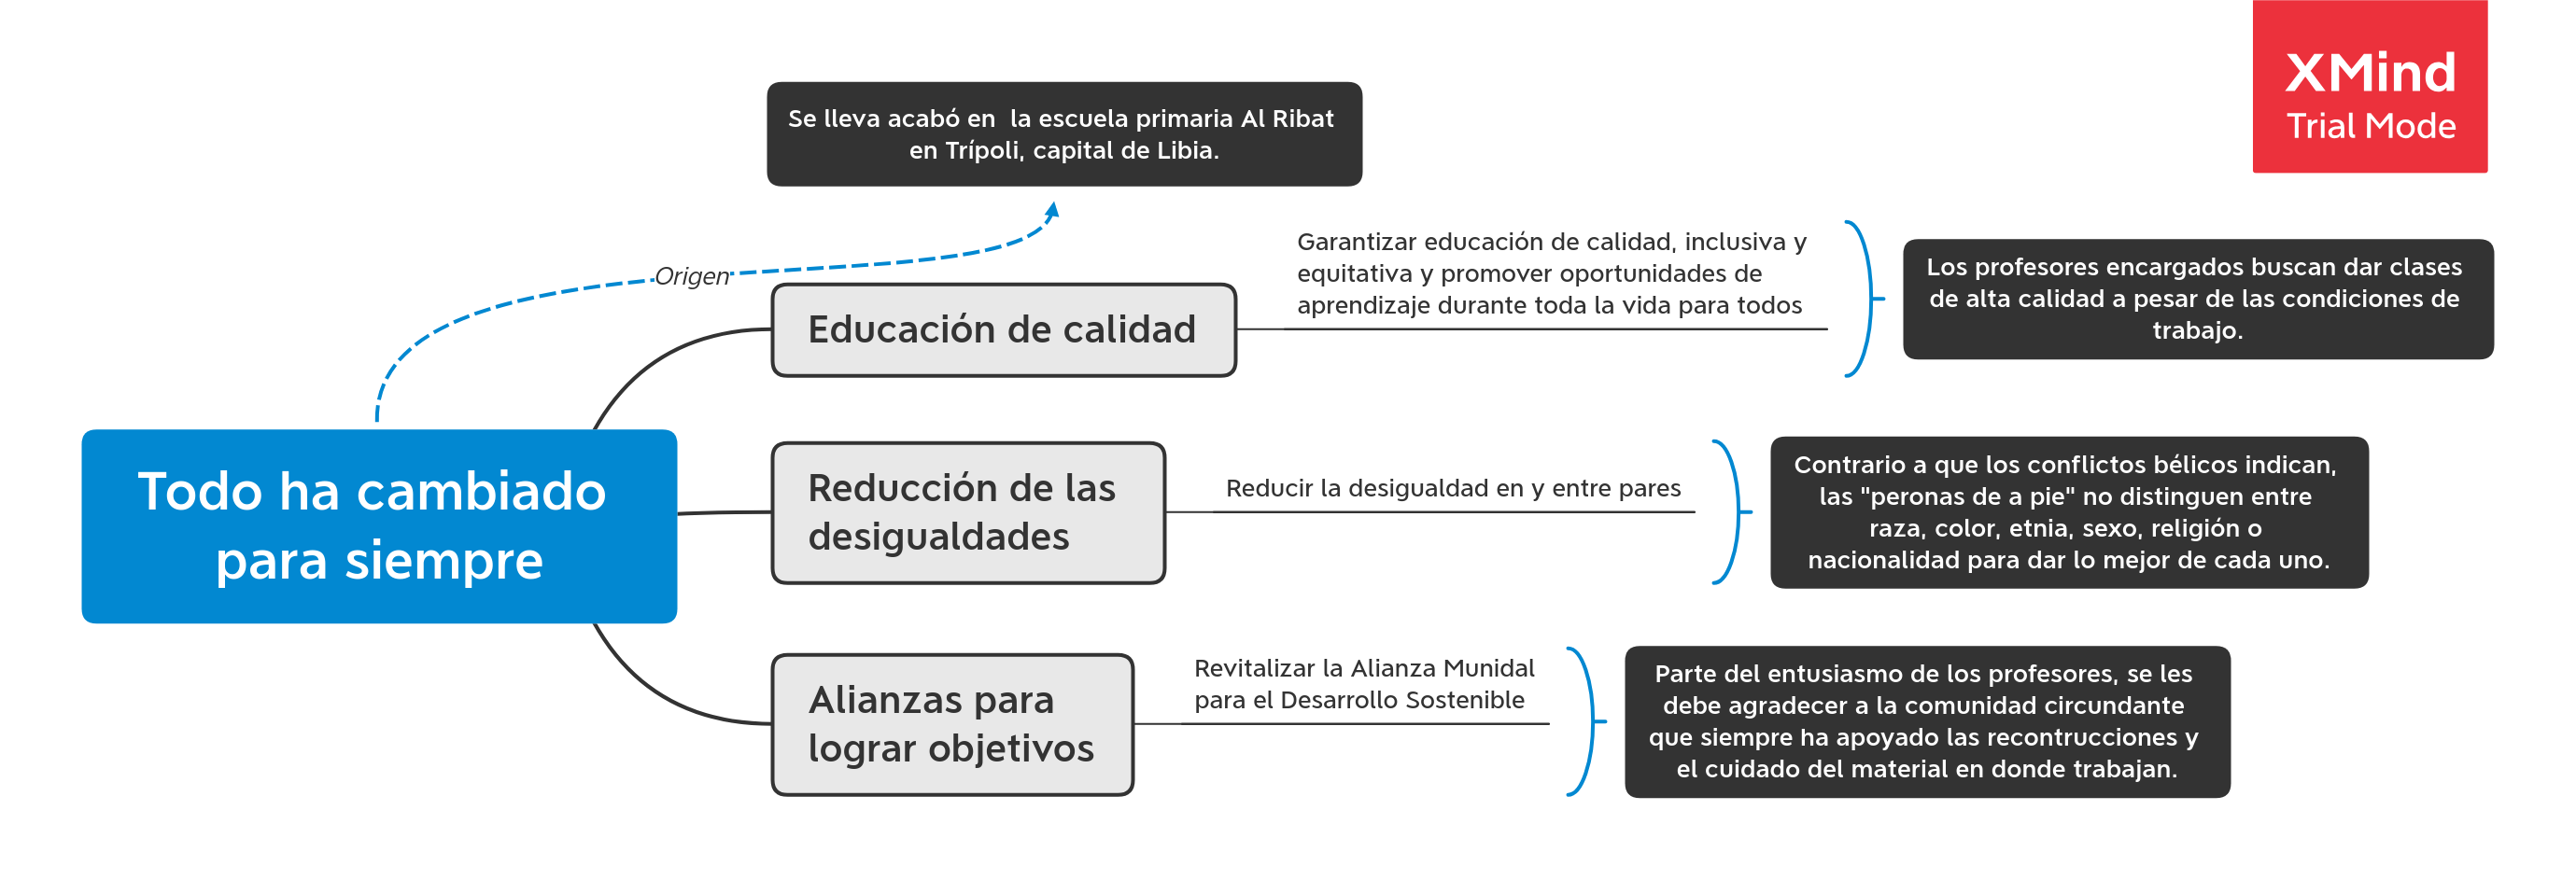
\includegraphics 
		[width=\textheight, height=0.8\textwidth, angle=90] 
		{BDSU-U2-A3-1.png}
	\caption{Diagrama de dimensiones del proyecto. El diagrama puede ser visualizado en una mayor resolución \href{https://github.com/BenchHPZ/UnADM-Biotecnologia/tree/master/B1-1/BDSU/Actividades/assets/BDSU-U2-A3-1.png}{aqui}}
\end{figure}


%%%%%%%%%%%%%%%%%%%%%%%%%%%%%%%%
%%         Bibliografia        %%
%%%%%%%%%%%%%%%%%%%%%%%%%%%%%%%%%%

\begin{thebibliography}{X}
	\bibitem{oficial} S/D. (2020). \textit{U2 $|$ Dimensiones y retos de la sustentabilidad}. 27 de julio de 2020, de UnADM Sitio web: \url{https://dmd.unadmexico.mx/contenidos/DCSBA/BLOQUE1/BI/01/BDSU/unidad_02/descargables/BDSU_U2_Contenido.pdf}
	\bibitem{objetivos} S/D. (S/D). \textit{Objetivo 4: Educación de calidad}. 27 de julio de 2020, de PNUD Sitio web: \url{https://www.mx.undp.org/content/mexico/es/home/sustainable-development-goals/goal-4-quality-education.html}
	\bibitem{agua} ONU Desarrollo. (2019). \textit{Todo ha cambiado para siempre}. 27 de julio de 2020, de Medium Sitio web: \url{https://medium.com/@pnud/todo-ha-cambiado-para-siempre-fa98dfdf4bce}
	\bibitem{github} BenchHPZ. (2020). UnADM-Biotecnología. 28 de Julio de 2020, de GitHub Sitio web: \url{https://github.com/BenchHPZ/UnADM-Biotecnologia/tree/master/B1-1/BDSU}


\end{thebibliography}
\end{document}